%\documentclass[english,12pt,a4paper,final]{article}
%\usepackage[T1]{fontenc}
%\usepackage[left=2cm, right=2cm, top=2cm, bottom=2cm]{geometry}
%\usepackage{amssymb,graphicx,amsfonts,amsthm, tikz, listings}
%\usepackage{bookman}
%\usepackage[bahasa]{babel}
%\usetikzlibrary{shapes.geometric, arrows}
%\begin{document}
%	\begin{titlepage}
%		\centering
%		% TODO: \usepackage{graphicx} required
%		
\includegraphics[width=0.15\textwidth]{logounesa.png}\par\vspace{1cm}
%		{\large\textsc{Program Studi S1 Matematika} \par}
%		\vspace{1cm}
%		{\Large \textsc{Laporan Tugas}\par}
%		\vspace{1.5cm}
%		{\huge\bfseries Bahasa Pemrograman\par}
%		{\Large \textsc{4420102177}\par}
%		\vspace{2cm}
%		Oleh:\\
%		{\Large\itshape Masukkan Nama Anda\par}
%		22030214XXX\\
%		MA - 2022X
%		\vfill
%		Dosen Pengampu:\par
%		Dimas Avian \textsc{Maulana}, M.Si.\\
%		Riska Wahyu \textsc{Romadhonia}, S.Si., M.Sc. 
%		
%		\vfill
%		Ko-Asisten:\par
%		Masukkan Nama Ko-As Anda
%		\vfill
%		% Bottom of the page
%		{\large \today\par}
%	\end{titlepage}
%\section{Permasalahan}
%Uraikan masalah/tugas yang sedang Anda selesaikan disini
%\section{Diagram Alir}
%Buat Diagram alir disini. Berikut adalah contoh diagram Alir:
%\begin{center}
%	\begin{figure}[h!]
%		\tikzstyle{startstop} = [rectangle, rounded corners=0.5cm, minimum width=2.5cm, minimum height=1cm, text centered, draw=black]
%	\tikzstyle{io} = [trapezium, trapezium stretches=true, trapezium left angle=70,  trapezium right angle=110, minimum height=1cm, text centered, draw=black]
%	\tikzstyle{process} = [rectangle, minimum width=3cm, minimum height=1cm, text centered, draw=black]
%	\tikzstyle{decision} = [diamond, minimum height=1cm, aspect=2.5, text centered, draw=black]
%	\tikzstyle{arrow} = [ultra thick,->,>=stealth]
%	
%	\begin{tikzpicture}[node distance=2.25cm]
%		\node (start) [startstop] {Mulai};
%		\node (in) [io, below of=start] {Data Saham};
%		\node (pro2) [decision, below of=in] {Input Parameter};
%		\node (pro3) [process, below of=pro2] {Hitung nilai $dt, u, d, p, v_{es}$ dan $S_{ij}$};
%		\node (pro4) [process, below of=pro3] {Menghitung harga opsi saat jatuh tempo};
%		\node (pro5) [process, below of=pro4] {Melakukan hitung mundur seperti metode Binomial untuk memperoleh $f_{0,0}$};
%		\node (stop) [startstop, below of=pro5] {Selesai};
%		
%		\draw [arrow] (start) -- (in);
%		\draw [arrow] (in) -- (pro2);
%		\draw [arrow] (pro2) -- (pro3);
%		\draw [arrow] (pro3) -- (pro4);
%		\draw [arrow] (pro4) -- (pro5);
%		\draw [arrow] (pro5) -- (stop);		
%	\end{tikzpicture}
%		\caption{Alur penelitian}
%	\end{figure}
%\end{center}
%\section{\textit{Source Code}}
%Tuliskan \textit{source code} disini. Berikut adalah contoh \textit{source code}:
%\lstinputlisting[language=python]{epidemiology.py} %ganti epidemiology.py dengan file Anda
%
%\section{Tangkapan Layar Hasil \textit{Running Source Code}}
%\begin{figure}
%	\centering
%	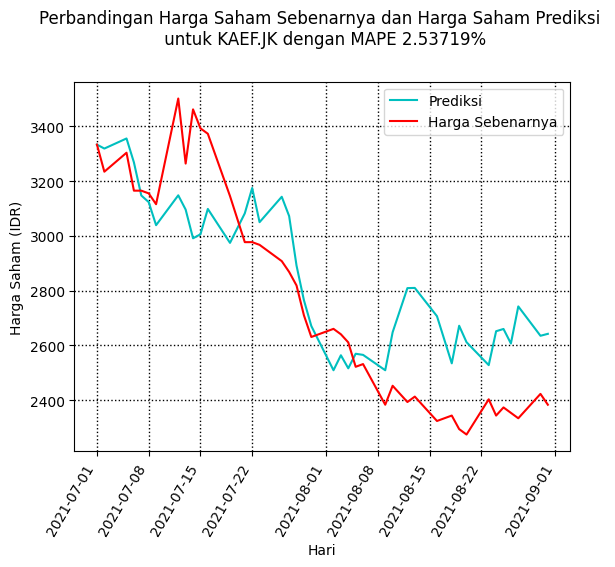
\includegraphics[width=\linewidth]{KAEF}
%	\caption{Hasil running program dengan input xxx}
%	\label{fig:kaef}
%\end{figure}
%
%\section{Penjelasan}
%Berikan penjelasan terhadap program yang Anda kerjakan.
%
%\begin{thebibliography}{9} 
%	\bibitem{Azuela} Mariano Azuela, \textit{The Underdogs: A Novel of the Mexican Revolution}, trans. Beth Jorgensen (New York: The Modern Library, 2002). 
%\end{thebibliography}
%\end{document}